% !TEX root = diplomarbeit.tex
\chapter{Kommunikation Applikation und Hexacopter}
\renewcommand{\kapitelautor}{Autor: Katharina Joksch, Lucas Ullrich}
Um zwischen dem Hexacopter und dem Server eine Verbindung herzustellen wird eine Kommunikationsschnittstelle benötigt. Diese muss drahtlos arbeiten und einen größeren Bereich
abdecken. Über diese werden anschließend die diversen Daten übertragen, dazu zählen zum Beispiel die Route, beziehungsweise der Name des Gastes.

%%%%%%%%%%%%%%%%%%%%%%%%%%%%%%%%%%%%%%%%%%%%%%%%%%%%%%%%%%%%%%%%%%%%%%%%%%%%%%%
\section{Allgemeine technische Planung}
Autor: Lucas Ullrich\\ \\
In der Planung wurde eine unkomplizierte und verlässliche Lösung für beide Kommunikationspartner gesucht. Da Bluetooth kaum noch standardmäßig verbaut ist, wird hier wiederum
serverseitig eine externe Hardware benötigt, um dies zu vermeiden wurde WLAN ins Auge gefasst.

WLAN stellte sich folglich als ideale Schnittstelle heraus,
es gibt die Möglichkeit für ein Handover (Verbindungsübergabe) in sehr großen Bereichen, es ist nach einmaligem Setup vergleichsweise unkompliziert und es bietet diverse
Möglichkeiten, festzustellen ob die Verbindung noch aufrecht ist.

      \subsection{Kommunikationsschema}
Für die Kommunikation zwischen dem Hexacopter und dem Server wurde folgendes Schema festgelegt:
\begin{table}[H]
\centering
\begin{tabular}{|p{0.5cm}|p{2cm}|p{2cm}|p{5.5cm}|p{2cm}|}
\hline \textbf{ID} & \textbf{Von wem?} & \textbf{Was?} & \textbf{Wann?} & \textbf{An wen?} \\\hline
\hline 1 & WLAN-Modul & 1 & wenn er in der Basis ist bzw. \newline bereit ist eine Speise auszuliefern & Server \\\hline
\hline 2 & Server & 2 & alle zwei Sekunden & WLAN-Modul \\\hline
\hline 3 & Server & Tischroute & sobald er eine Nachricht mit dem Inhalt "1" erhält & WLAN-Modul \\\hline
\end{tabular}
\caption{Kommunikationsschema - Hexacopter und Server}
\end{table}

\begin{itemize}
    \item \textbf{ID 1}\\
Damit der Server weiß, wann der Hexacopter sich in der Basis befindet und dadurch bereit ist eine Speise auszuliefern, schickt der Mikroprozessor über WLAN einen Einser.

    \item \textbf{ID 2}\\
Damit kontrolliert werden kann, ob die Verbindung zu dem Hexacopter in Takt ist, wird im alle zwei Minuten ein Zweier geschickt.

    \item \textbf{ID 3}\\
Sobald der Server einen Einser von dem Hexacopter geschickt bekommt, sendet er ihm automatisch die Tischroute des Gastes, welcher als nächstes seine Bestellung erhalten soll.
Die Tischroute ist mit folgendem Schema aufgebaut: \\
"$<<$ Farbcode Farbcode GS Farbcode $>>$" \\
Die Zeichen "$<<$" zeigen dem WLAN-Modul, dass eine Nachricht beginnt.
Anschließend werden die Farbcodes welche sich auf dem Bodenbefinden versendet.
Das Kürzel "GS" steht für "Group seperator" und hilft dem Modul die Farbcodes zwischen Boden und Tisch zu unterteilen.
Am Ende der Tischroute werden dem Hexacopter noch die Zeichen "$>>$" geschickt, damit er weiß, dass die Route fertig gesendet wurde.
Die einzelnen Zeichen werden dem WLAN-Modul in der ASCII-Codierung übermittelt, die Leerzeichen vernachlässigt.
  \end{itemize}

%%%%%%%%%%%%%%%%%%%%%%%%%%%%%%%%%%%%%%%%%%%%%%%%%%%%%%%%%%%%%%%%%%%%%%%%%%%%%%%
\section{Schnittstelle Hexacopter}
Autor: Lucas Ullrich\\ \\
Seitens des Hexacopters wird ein zusätzliches Modul benötigt, dieses muss über eine der Schnittstellen des Mikrocontrollers ansprechbar sein.

  \subsection{Technische Planung}
  Bei der Planung wurde darauf geachtet ein WLAN-Modul zu wählen, welches bekanntermaßen funktioniert beziehungsweise ein entsprechender Support zur Verfügung steht.
  So fiel die Wahl auf das WLAN-Modul RN171, vertrieben durch Microchip, hergestellt von Roving Networks.

  Das gewählte WLAN-Modul wird über eine UART-Schnittstelle angesteuert und verfügt über einige frei konfigurierbare Pins, diese werden schließlich zum Überwachen der
  Verbindung verwendet.

  \subsection{Umsetzung}
  Bei der Umsetzung stand, für die anfänglichen Tests, ein Evaluation-Kit zur Verfügung. Dieses kann ohne weitere Hardware direkt über ein USB-Kabel mit einem PC verbunden werden.
  So ist es möglich, die nötigen Konfigurationen des Moduls auszutesten, bevor dieses in der Hardware implementiert wird.

  \begin{figure}[H]
    \begin{centering}
      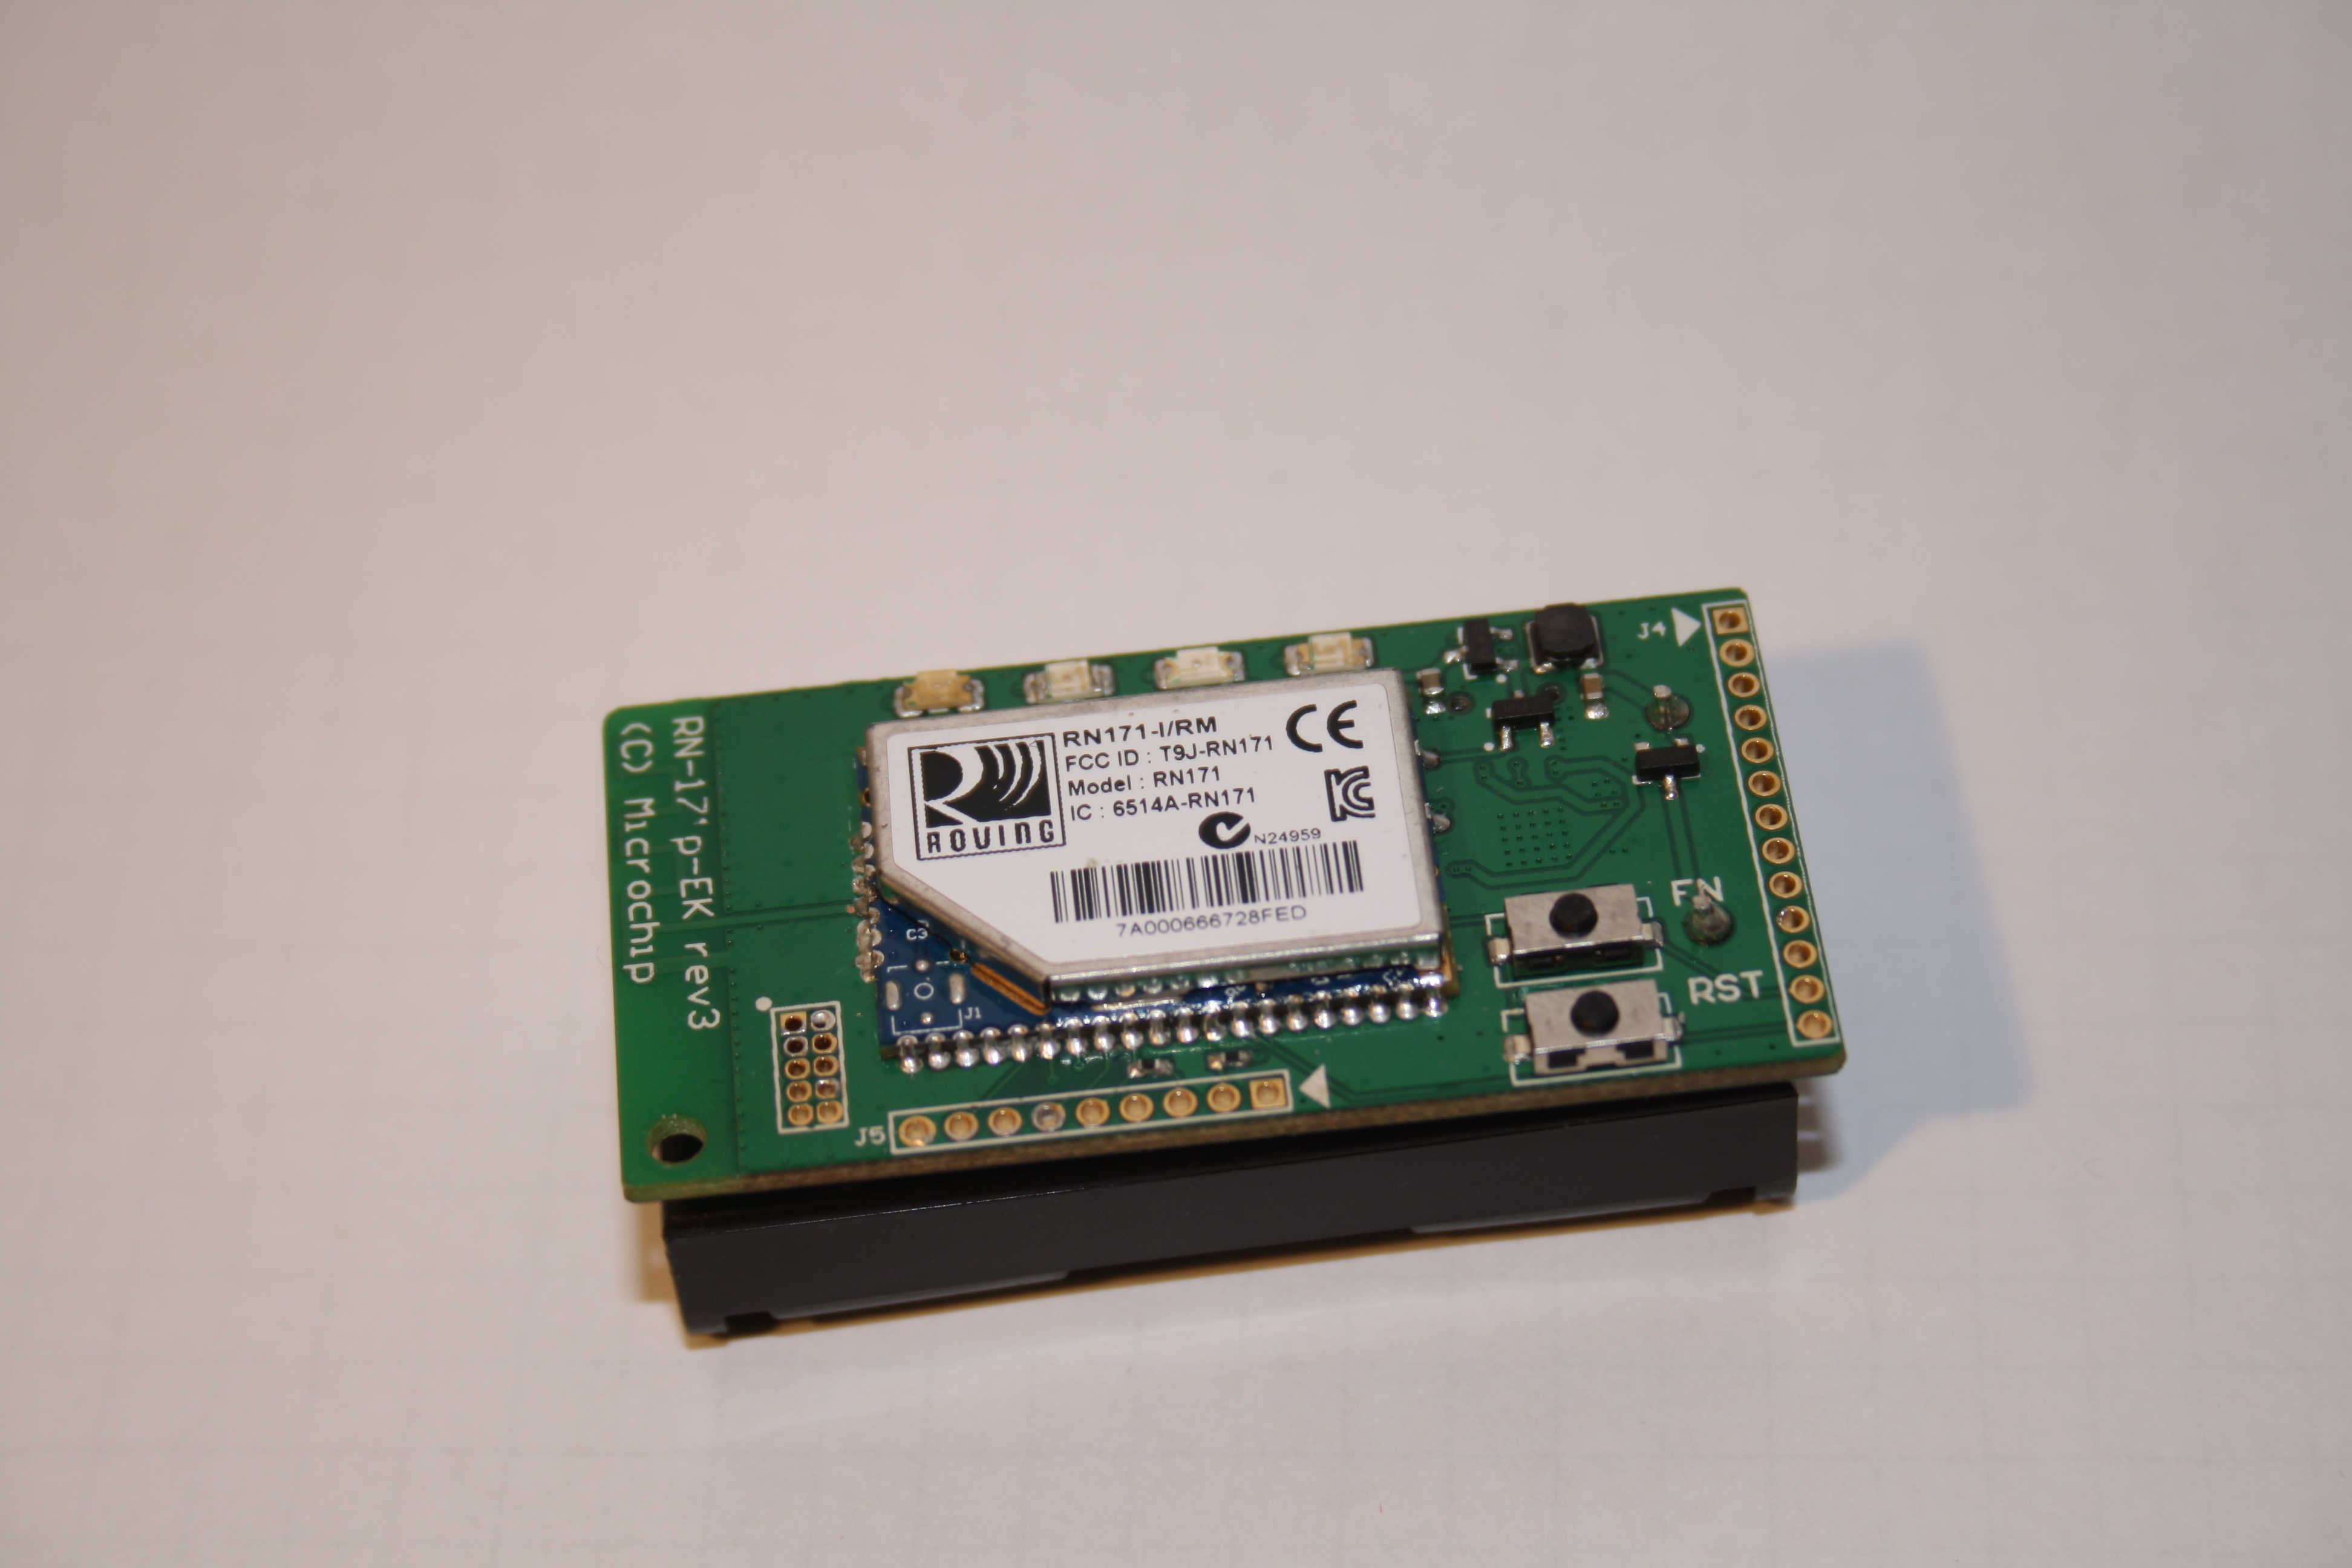
\includegraphics[width = 0.6\textwidth]{Bilder/RN171_EK}
    \par\end{centering}
    \caption[RN171 Evaluation-Kit]{RN171 Evaluation-Kit}
    \label{RN171_EK}
  \end{figure}

Um das WLAN-Modul so einzustellen, dass es sich Pin-gesteuert mit einem Host verbindet sind einige Schritte notwendig:
  \begin{itemize}
    \item \textbf{\$\$\$}\\
    Öffnet den Commandmode, nun können die Einstellungen vorgenommen werden
    \item \textbf{set wlan ssid <network\_name>}\\
    Deklariert den Netzwerknamen
    \item \textbf{set wlan phrase <network\_passphrase>}\\
    Deklariert das Passwort mit dem das Netzwerk gesichert ist
    \item \textbf{set ip host <host\_ip-address>}\\
    Deklariert die IP-Adresse des Empfängers
    \item \textbf{set ip remote <host\_portnumber>}\\
    Deklariert den Port auf dem der Empfänger die Daten empfangen soll
    \item \textbf{set sys iofunc 0x70}\\
    Durch diese Einstellung kann das WLAN-Modul über die Pins gesteuert werden
    \item \textbf{set wlan join 1}\\
    Stellt das WLAN-Modul auf automatisches Verbinden mit dem angegebenen Netzwerk ein
    \item \textbf{set ip protocol 4}\\
    Stellt das WLAN-Modul auf eine TCP/IP-Verbindung ein bei der nur Daten vom gespeicherten Host akzeptiert werden
    \item \textbf{set uart baud <desired-baudrate>}\\
    Stellt die Baudrate des WLAN-Moduls ein, Standard ist 9600
    \item \textbf{save}\\
    Speichert die Parameter in den Standardeinstellungen die nach einem Neustart geladen werden
    \item \textbf{reboot}\\
    Erzeugt einen Neustart bei dem die Standardeinstellungen geladen werden
  \end{itemize}
  Nachdem das WLAN-Modul auf die nötigen Parameter eingestellt ist, kann es direkt mit dem Mikrocontroller verbunden werden, die Verbindung kann über einzelne Pins kontrolliert
  werden.

  \subsection{Herausforderungen und Lösungen}
  Eine Herausforderung stellte die Frage dar, wie genau die Verbindung hergestellt wird. Das Datenblatt des WLAN-Moduls, mit über 100 Seiten, bietet viele potentielle Möglichkeiten.
  Die erste Wahl fiel auf das Auslesen einer Website, auf den ersten Anblick funktionierte das auch, jedoch musste festgestellt werden, dass unabhängig von der Website sehr ähnliche
  Daten verarbeitet werden, jedoch nicht der eigentliche Inhalt der Website sondern Providerinformationen.

  Die zweite Wahl fiel auf eine TCP/IP Verbindung, lediglich die genaue Umsetzung dieser, ließ viele Möglichkeiten offen. Einerseits besteht die Möglichkeit eine Verbindung direkt
  über die Eingabe "open" im Commandmode zu öffnen, andererseits jedoch auch über die Pins als auch automatische Timeouts.

  Aufgrund der Einfachheit und vollen Kontrolle fiel die Wahl auf die Ansteuerung über die Pins.
  Dazu stehen 3 unterschiedliche Pins zur Verfügung:
  \begin{itemize}
    \item \textbf{Associated}\\
    Mit einem Netzwerk verbunden
    \item \textbf{Open TCP connection}\\
    Die Verbindung zum Host herstellen
    \item \textbf{Connected}\\
    Die Verbindung zum Host ist hergestellt
  \end{itemize}
  Die Statusinformationen "Associated" als auch "Connected" werden von dem WLAN-Modul geliefert, die Anweisung eine Verbindung herzustellen von dem Mirkocontroller.

%%%%%%%%%%%%%%%%%%%%%%%%%%%%%%%%%%%%%%%%%%%%%%%%%%%%%%%%%%%%%%%%%%%%%%%%%%%%%%%
\pagebreak
\section{Schnittstelle Applikation}
Autor: Katharina Joksch\\

  \subsection{Technische Planung}

	   \subsubsection{JDBC}

Die Java Datenbankschnittstelle {JDBC\cite{jdbc}} ist ein Industriestandard für datenbankunabhängige Verbindungen zwischen Java Programmen, SQL Datenbanken und sämtlichen anderen tabellenbasierten Datenbankmodellen. Zu den Aufgaben von JDBC gehört es, Datenbankverbindungen aufzubauen und diese zu verwalten. Außerdem kann JDBC  SQL-Anfragen an die Datenbank weiterleiten, Ergebnisse in eine für Java nutzbare Form umwandeln und diese dem Programm zur Verfügung stellen.

	   \subsubsection{Zusammenspiel mit der Applikation und dem WLAN-Modul}
Das Java-Programm und die Applikation kommunizieren nur indirekt miteinander, da beide nur auf die Datenbank zugreifen, um deren Inhalt zu überprüfen und Einträge upzudaten beziehungsweise zu erstellen.
Mit dem WLAN-Modul wird hingegen auf direktem Weg kommuniziert.
			\begin{figure}[H]
			\begin{centering}
			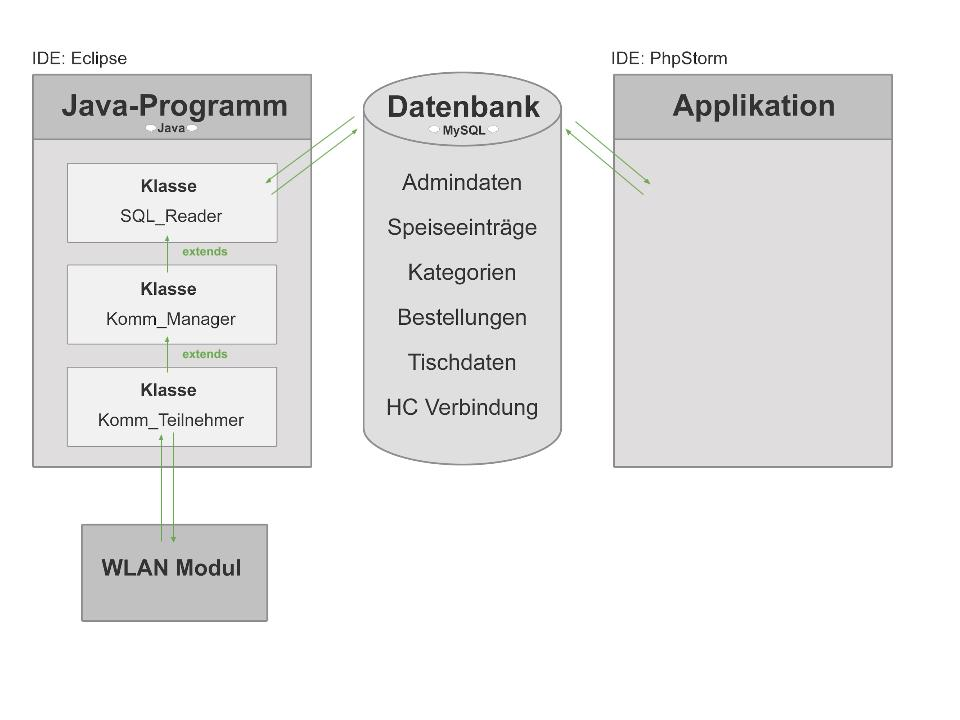
\includegraphics[width = 1\textwidth]{Bilder/Jok_zusammenspiel_java.jpg}
			\par\end{centering}
			\caption{neue MockUps - Admininterface}
			\label{neue MockUps - Admininterface}
			\end{figure}

      \subsubsection{Eclipse}

Eclipse ist eine freie Entwicklungsumgebung für Programme und wurde von der Eclipse Foundation entwickelt. Das Programm kann verwendet werden, um in mehreren Programmiersprachen Software zu entwickeln. Besonders gut geeignet ist Eclipse für die Entwicklung von Java-Programmen, da es sowohl Auto-Completion ermöglicht als auch Syntax-Hervorhebung.

  \subsection{Umsetzung}
Für die Umsetzung des Javaprogramms wurden drei verschiedene Klassen erstellt:\\ \\
\textbf{SQL Reader}\\
Diese Klasse wurde dazu programmiert, alle Datenbankzugriffe zu regeln.
Um den {Zugriff auf Datenbanken zu bewerkstelligen wurde JDBC\cite{jdbctutorial}} verwendet.
Damit das Programm mit JDBC arbeiten kann musste es zuerst von Oracle gedownloadet und anschließend mit einem Rechtsklick auf das Javaprojekt unter dem Menüpunkt "Properties" als Bibliothek angeben werden.
\\ \\
Wie auch bei Doctrine müssen der Datenbank-Host, der Datenbank-Port und die Benutzerdaten angegeben werden, damit die Verbindung hergestellt werden kann.
Als Treiber wird hier jedoch statt MySQL auf JDBC verwiesen.
Um die Verbindung herzustellen wurde die Funktion DriverManager.getConnection() aufgerufen. Als Parameter mussten ihr der Pfad zur Datenbank und die Benutzerdaten mitgeschickt werden.
\lstset{language = java}
  	\begin{lstlisting}
private String db_host = "localhost";
private String db_port = "3306";
private String db_user = "root";
private String db_pass = "root";
private String db_base = "DbSpeisekarte";
private static final String DRIVER = "com.mysql.jdbc.Driver";

//...

String mySqlUrl = "jdbc:mysql://" + db_host + ":" + db_port + "/"
+ db_base;

verbindung = DriverManager.getConnection(mySqlUrl, db_user, db_pass);
	\end{lstlisting}
Damit die Tischdaten angezeigt werden konnten, wurde die "showTischdaten()"-Funktion erstellt. Um die ID, die Tischroute und die Tischnummer zu erhalten musste jeweils ein SQL-Statement verfasst werden. In diesem SQL-Statement wurden nur die Tischdaten, welche einer Bestellung zugeordnet sind ausgelesen.
Um das Statement anschließend auszuführen, wurde es der vordefinierten Methode "executeQuery()" als Parameter mitgeschickt.
Die Ergebnisse werden in ein ResultSet gespeichert. Danach werden sie in einer Schleife iteriert und der aktuelle Wert aus dem Set als String umgewandelt. Nun konnte die Route als Rückgabewert angegeben werden.
\\ \\
Damit in der Bestellungen-Tabelle angemerkt wird, wann die Bestellung ausgeliefert wurde, wird mit SQL ein Update-Statement erzeugt und mit der vordefinierten "executeUpdate()"-Funktion ausgeführt.
\\ \\
Um in einer extra Datenbanktabelle den Verbindungsstatus zwischen dem Hexacopter und dem Server überprüfen zu können, wird bei jeder Statusänderung die "erstelleDBEintrag()"-Funktion aufgerufen. Das Einfügen von Datenbankeinträgen kann mit einem Insert-Statement erledigt werden. Dieses muss im Anschluss ebenfalls mit der "executeUpdate()"-Methode durchgeführt werden.
\\ \\
\subsubsection*{Komm Manager}
Um die Verbindung mit dem Hexacopter zu managen wurde die "Komm Manager" Klasse programmiert.
Damit diese Klasse die Funktionen der "SQL Reader"-Klasse verwenden kann, erbt sie von dieser. Dies wird ganz oben bei der Klassendefinierung mithilfe des Befehls "extends" gehandhabt.
\\ \\
Als globale Variable wird ein Hashset, welches die Teilnehmer beinhaltet, erstellt.
Anschließend wird ein Server Socket erstellt, welchem später ein geeigneter Port zugewiesen wird.
\\ \\
Mithilfe eines Timers wird alle zwei Sekunden überprüft ob ein Teilnehmer vorhanden ist. Wenn das der Fall ist, wird auf eine Methode verwiesen, in welcher die Verbindung hergestellt und daher auch die SQl-Readerfunktion, welche einen neuen Datenbankeintrag erstellt, aufgerufen wird. Diese SQL-Readerfunktion erneuert daraufhin den Verbindungsstatus.
\\
Sobald ein Teilnehmer beitritt wird ihm mithilfe des Timers regelmäßig eine Nachricht, mit dem Inhalt "2", geschickt.
\\ \\
Um zu überprüfen, ob der Hexacopter in der Basis und somit bereit dazu ist, eine Speise auszuliefern, wartet der Server darauf, dass die Nachricht "1" geschickt wird. Sobald diese Nachricht ankommt, liefert die Funktion den Wert "true" zurück. Außerdem wird mithilfe der SQL-Readerfunktion in der Datenbank vermerk, dass sich der Hexacopter zu diesem Zeitpunkt in der Basis befindet.
\\ \\
\subsubsection*{Komm Teilnehmer}
Die "Komm Teilnehmer" Klasse wurde dafür entwickelt, die einzelnen Verbindungen zum Hexacopter zu verwalten.
\\
Dem Teilnehmer Thread wird sowohl der Manager als auch der Server Socket als Parameter mitgeliefert. Über diese kann im Anschluss das Senden und Empfangen der Nachrichten geregelt werden.
\\ \\
In dieser Klasse wird die Nachricht des Hexacopters an die Manager Funktion geschickt, welche überprüft ob die Nachricht aussagt, dass sich der Multicopter in der Basis befindet.
\\
Wenn das der Fall ist, wird automatisch die Tischnummer der auszuliefernden Bestellung über die "showTischdaten()"-Funktion der SQL-Reader Klasse abgerufen und an den Hexacopter geschickt.

  \subsection{Herausforderungen und Lösungen}
Beim Abruf der einzelnen Tischdaten kam ab und zu das Problem auf, dass bei den SQL-Statements vergessen wurde, einen Zeilenabstand zu machen, nachdem eine Variable eingebunden wurde. Dies waren jedoch nur kleine Fehler, die in der Eile entstanden und relativ schnell erörtert und ausgebessert werden konnten.
